% CREATED BY DAVID FRISK, 2016
\chapter{System Development}

\section{Overview}
As already mentioned, the use of custom hardware for a specific application can have big benefits especially in terms of energy consumption and latency.
The inference process of Neural Network is mainly characterized by massive multiply and addition operations. Fetch of data from main memory follows patterns and it has been proved that those data, in particular weight data, are reused for several executions of the Neural Network model.
As consequence, executing a Neural Network model on a von Neumann based architecture machine leads to performance degradation, even in a cache-based system, since the CPU has to request the data from the main memory, execute the operation on those data and then save back to main memory before moving to the next data. The introduction of vectored instruction in the modern processors can have a slight impact in the performance benefits. However, the drastically increase of layers in the Neural Network has made them suitable for several applications. This it can be translated into a massive increase of operations for executing them, as it can be also observed in the following Figure:
\begin{figure}[!htbp]
\centering
\captionsetup{justification=centering}
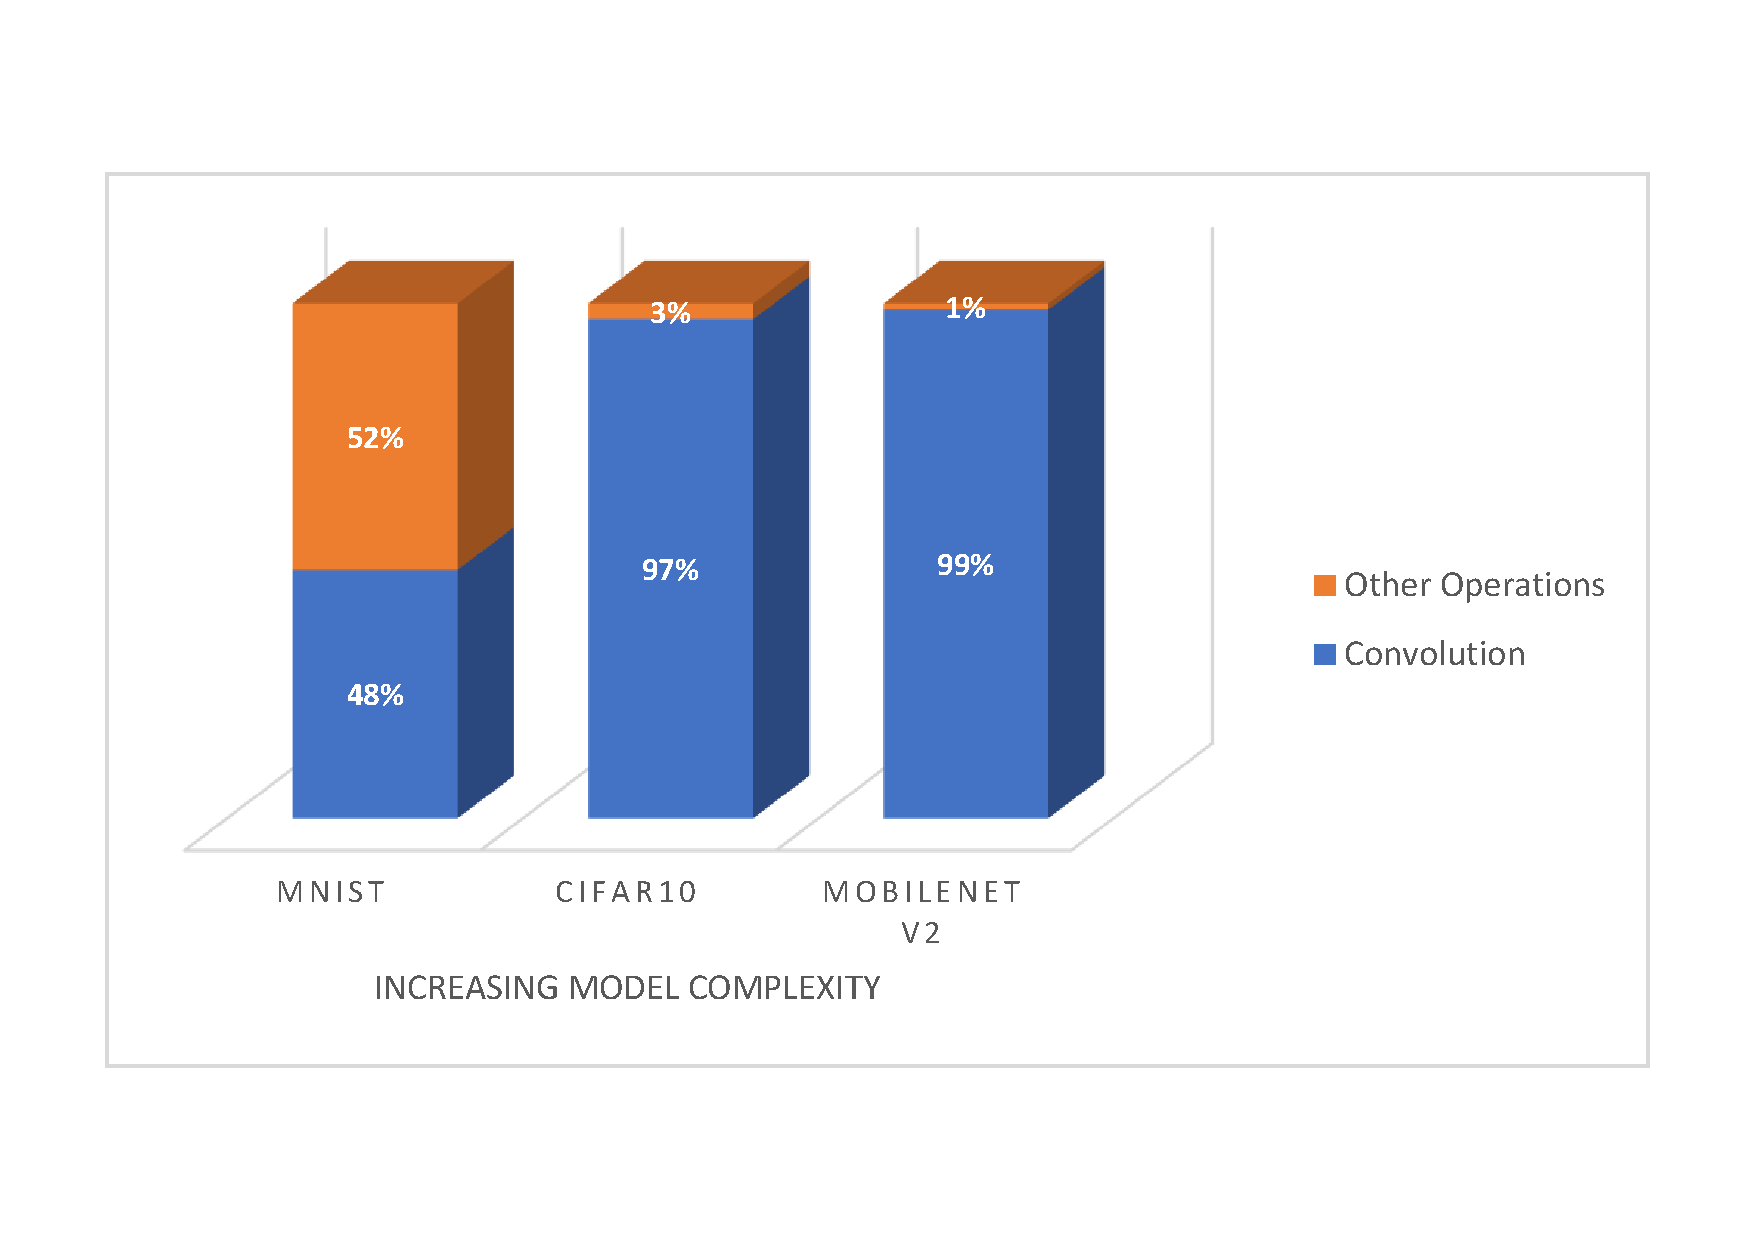
\includegraphics[scale=0.4]{./figure/exec_time.pdf}
\caption{Average execution time divided by type of operations}
\label{fig:exec}
\end{figure}

Following the fast demands of operations into a Neural Network, it becomes evident that executing them on a CPU could not meet real-time application requirements.\\
Instead, the designed accelerator has a Dataflow architecture, with emphasis on weight data reuse, and it is able to execute a tensor convolution. The basic idea is a computation matrix composed in every entry of processing elements which are able to perform operation between the incoming data and the weights, which have been already loaded for exploiting a data reuse approach.\\\\
The custom hardware accelerator is not useful as it is. It has to be integrated into a ML-Framework in order to appreciate its benefits. After a preliminary research on which ML-Framework would allow to integrate a custom hardware accelerator minimizing the efforts to change the model code and its definitions, it has been evident that the TensorFlow Framework, an end-to-end open source Machine Learning platform \cite{WEBSITE:4}, suits the needs.\\
\newpage
The workflow of the Hardware-Software development is illustrated in the following:
\begin{figure}[!htbp]
\centering
\captionsetup{justification=centering}
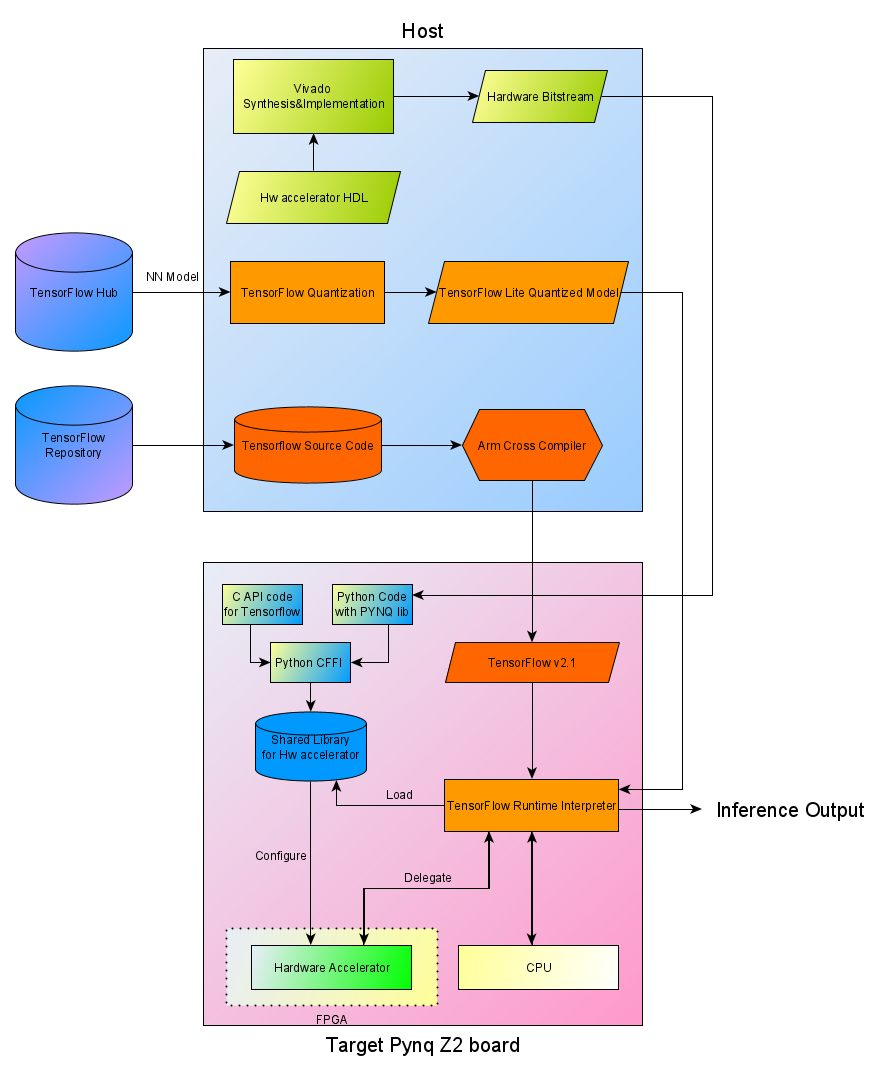
\includegraphics[scale=0.5]{./figure/workflow.png}
\caption{Development workflow}
\label{fig:workflow}
\end{figure}

\newpage
The entire work is implemented on a PYNQ Z2 board from TUL, based on a Zynq-7000 SoC \cite{paper:31}. In order to speed-up the development process and use built-in library for the AXI protocol and the DMA transfers, the software is partially carried out through the PYNQ environment of the board \cite{WEBSITE:2} based on Python which has became a de facto standard \cite{paper:37}. \\
The usage of Python as basic software allows to easily integrate it with high level Machine Learning Framework, such as TensorFlow in this case. 
\newpage
\section{Software}

The focus of the work is the inference process, pre-trained models are needed and TensorFlow Hub \cite{WEBSITE:5} comes in handy for this purpose. It provides already pre-trained Machine Learning models for different domains. Moreover, TensorFlow has the feature of quantizing a post-trained model for different arithmetic precision. In the Fig. \ref{fig:workflow} it can be seen that the quantization process has been done offline.\\
The choice of using the stable release 2.1 of TensorFlow is dictated from the possibility of using Delegates (aka hardware accelerators or GPUs) in its Neural Network model. A delegate is a way to delegate part or all graph execution to another executor. Every model is represented, internally, as a graph (with its relative order of execution for the nodes) and every node of the graph is described as a set of operation that has to be applied to the node's input. As every node is described by a set of operations, it is easy to understand which part of the graph can be executed on the accelerator in advance, and this operation is done at the beginning when both the model and the accelerator library is loaded as it is represented in the following Figures:
\begin{figure}[!htbp]
\captionsetup{justification=centering}
    \centering
    \subfloat[without delegate]{{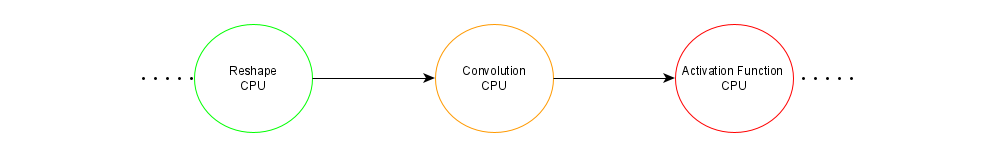
\includegraphics[scale=0.45]{./figure/exec_graph.PNG} }}%
    \qquad
    \centering
    \subfloat[with delegate]{{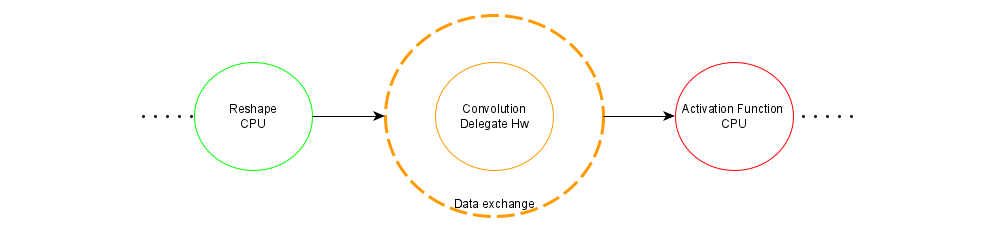
\includegraphics[scale=0.45]{./figure/exec_graph_delegate.PNG} }}%
    \caption{Execution Graph}%
    \label{fig:execgraph}%
\end{figure}
 It is worth to mention that TensorFlow is open-source and since no binary installations for its 2.1 release are provided for Arm processor, it has been cross-compiled from scratch for the PYNQ-Z2 board. 
 \newpage
TensorFlow demands as library for the accelerator a C Python-API compatible shared library. In addition, the code for using the accelerator was already written using the PYNQ environment in Python. Therefore, for allowing code reuse and decreasing the development time the Python code has been embedded in the C code (from a TensorFlow example of the delegate library), adding callbacks to Python code\footnote{See Appendix A}. This has been possible thanks to the Python library \textit{CFFI} (C Foreign Function Interface) \cite{WEBSITE:14}, which is also able to provide a shared library Python-API compatible as output. In the following Figure the flow chart between Tensorflow Lite and the accelerator library can be seen:
\begin{figure}[!htbp]
\centering
\captionsetup{justification=centering}
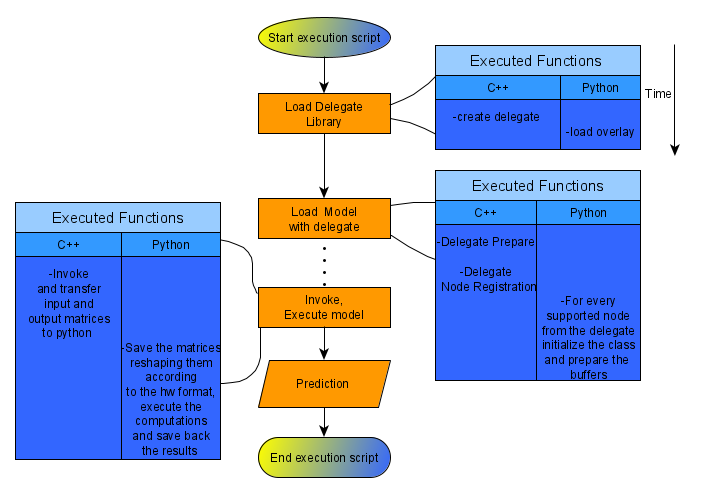
\includegraphics[scale=0.6]{./figure/flow_chart_accelerator.png}
\caption{Flow Chart with accelerator}
\label{fig:fcaccelerator}
\end{figure}

\newpage
\section{System Level}

As it can be seen from Figure \ref{fig:zynq}, it is divided in two big blocks:
\begin{itemize}
\item Processing System:
The processing system (in Figure \ref{fig:sys} referred as \textit{processing system7}) is in charge of running the OS and the Machine Learning application. As consequence it also runs the necessary software for programming the accelerator registers and the data movement to/from main memory from/to the accelerator.
\item Programmable Logic:
The programmable logic (PL) hosts the entire design, from the accelerator itself to the DMAs and the AXI interconnections.
\end{itemize}

\begin{figure}[!htbp]
\centering
\captionsetup{justification=centering}
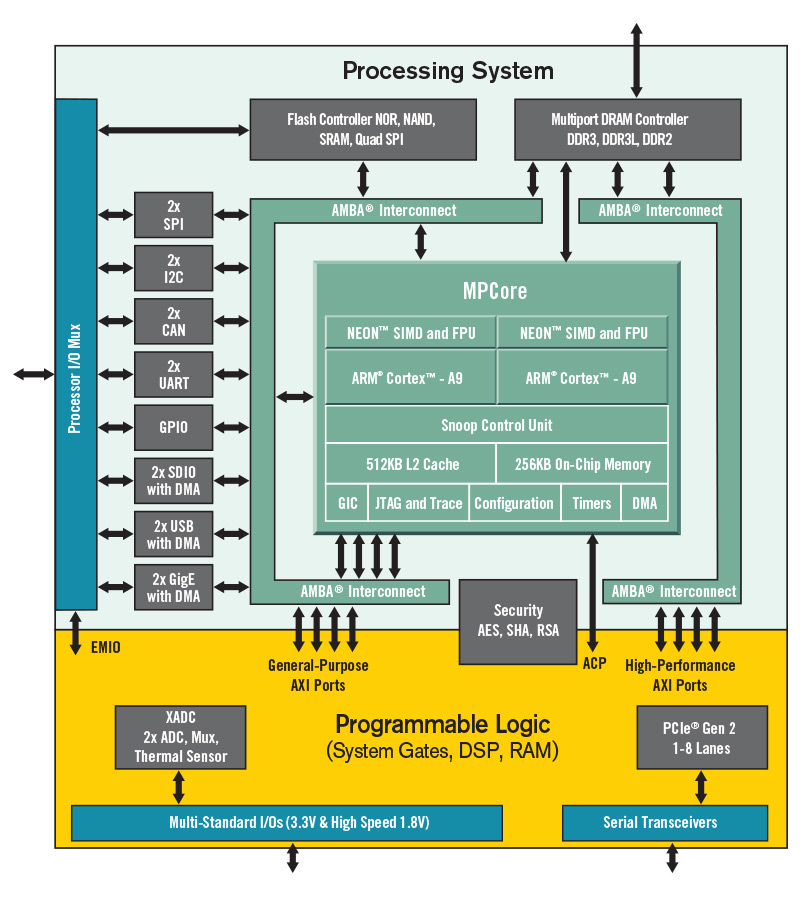
\includegraphics[scale=0.35]{./figure/zynq.PNG}
\caption{Zynq 7000 SoC \cite{paper:42}}
\label{fig:zynq}
\end{figure}

Furthermore, the Programmable Logic in Figure \ref{fig:sys} is hosting:
\begin{itemize}
\item AXI interconnections: IP cores from Xilinx \cite{paper:34} \cite{paper:35} in order to connect and correctly address entities in the Programmable Logic.
\item AXI DMA: IP core from Xilinx \cite{paper:33} which allows data movement between main memory and accelerator memories.  Several single channel DMA have been used instead of using a single DMA with multiple channels. The reason is that in the PYNQ environment only the drivers for the single channel DMA are provided. 
\item DTPU: the actual hardware accelerator.
\item XADC: IP core from Xilinx \cite{paper:32} which allows to measure the temperature of the SoC, the voltages and the currents at run time.

\end{itemize}

\newpage
In the following figure, the schematic of the overall design in the PL is presented.
\begin{figure}[!htbp]
\centering
\captionsetup{justification=centering}
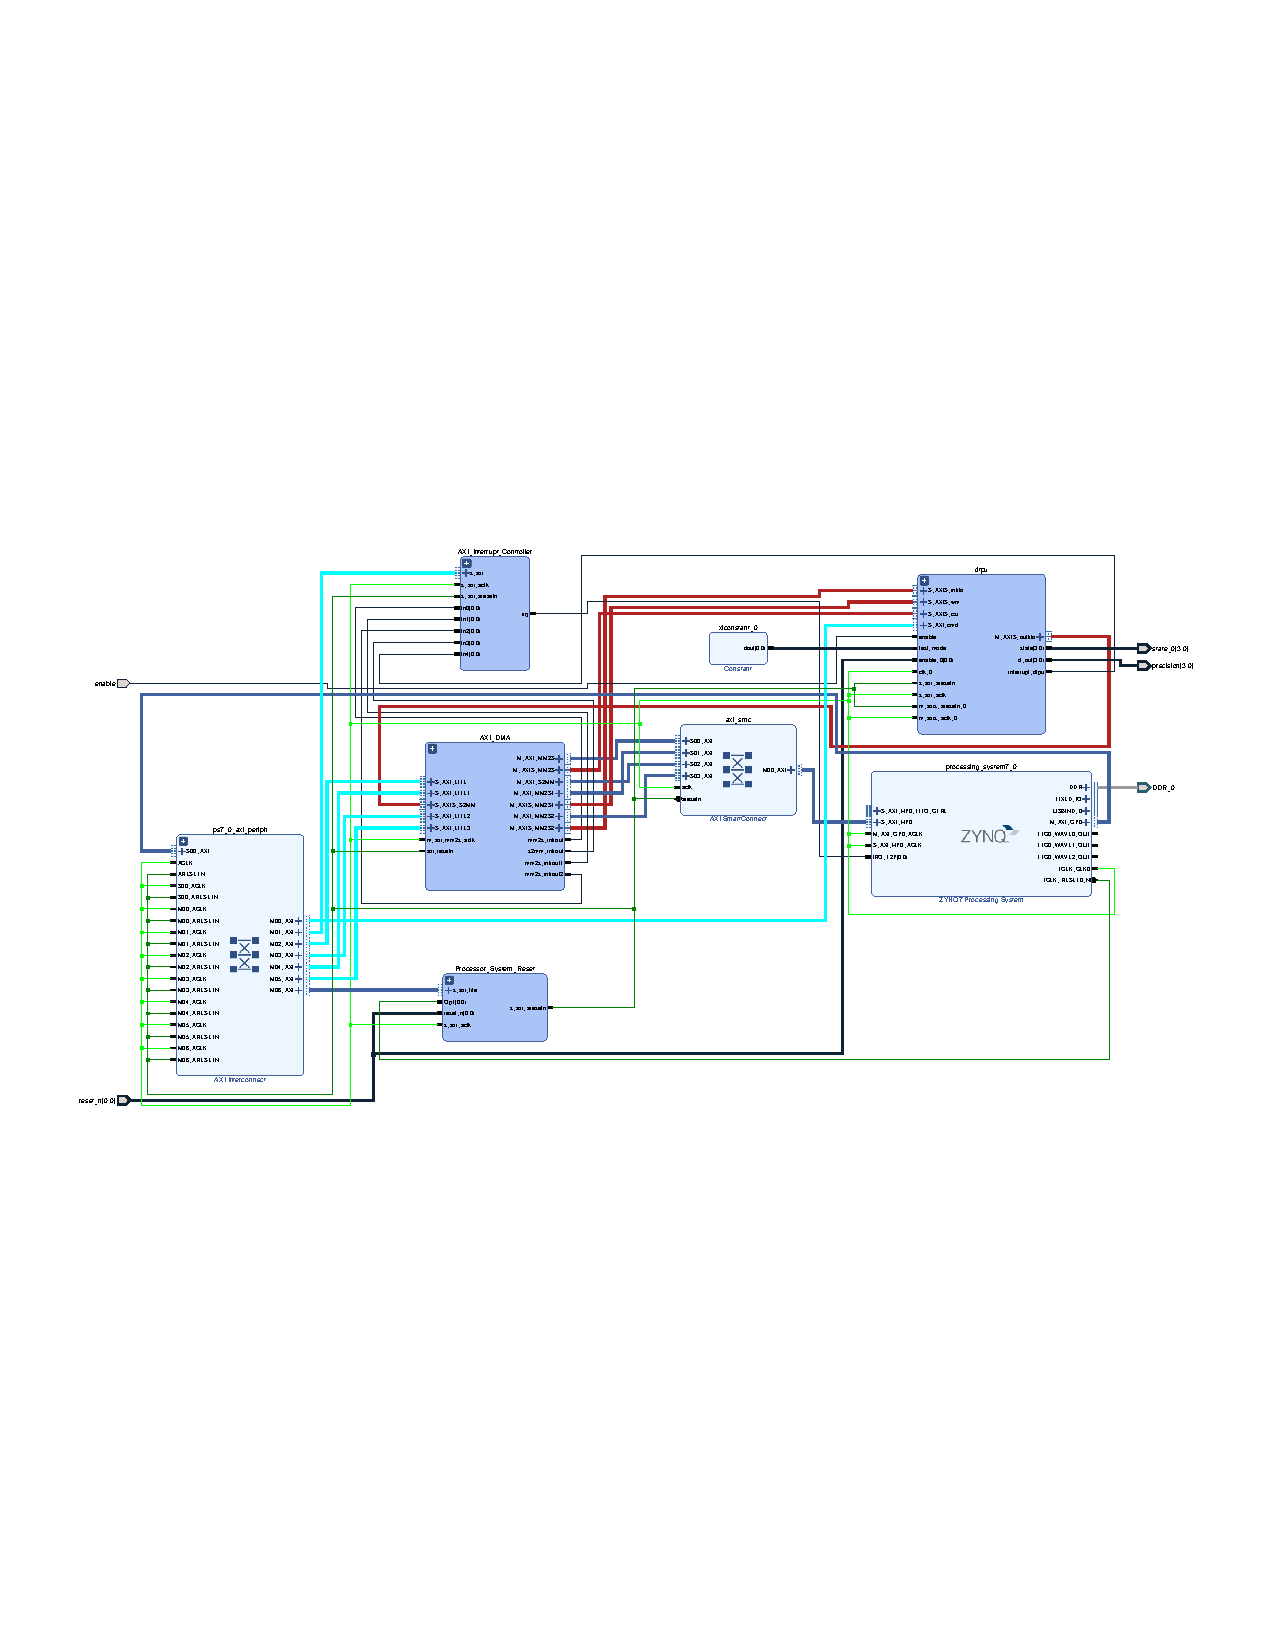
\includegraphics[scale=1,angle=90]{./figure/system_schematic.pdf}
\caption{System view hosted in the PL \protect\footnotemark}
\label{fig:sys}
\end{figure}
\footnotetext{Except for the Zynq Processing system}
\section{DTPU, the hardware accelerator}
The hardware accelerator, named \textit{Cogitantium\footnote{Thoughtful}, The Dumb Tensor Processing Unit}, is in charge of carrying out the tensor convolution of the neural network model, exploiting a data-flow architecture on the input data and a data reuse for the weight data.

Figure \ref{fig:logaccel} presents the Logical block diagram of the accelerator.
\begin{figure}[!htbp]
\centering
\captionsetup{justification=centering}
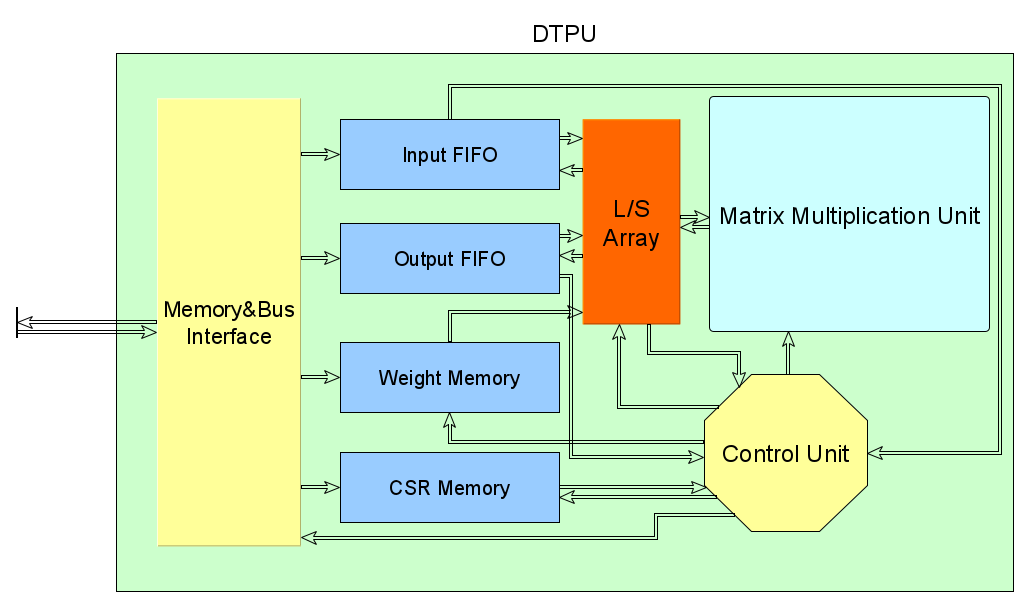
\includegraphics[scale=0.3]{./figure/logical_view.png}
\caption{Logical view of DTPU accelerator}
\label{fig:logaccel}
\end{figure}
\subsection{Real Implementation}
The work is not focused on developing embedded memories and AXI interfaces, therefore a Xilinx's IP core, which includes all those necessary sub components, has been used \cite{paper:43} leading to the actual block diagram which can be observed in the Figure \ref{fig:rtlaccel}.
\begin{figure}[H]
\centering
\captionsetup{justification=centering}
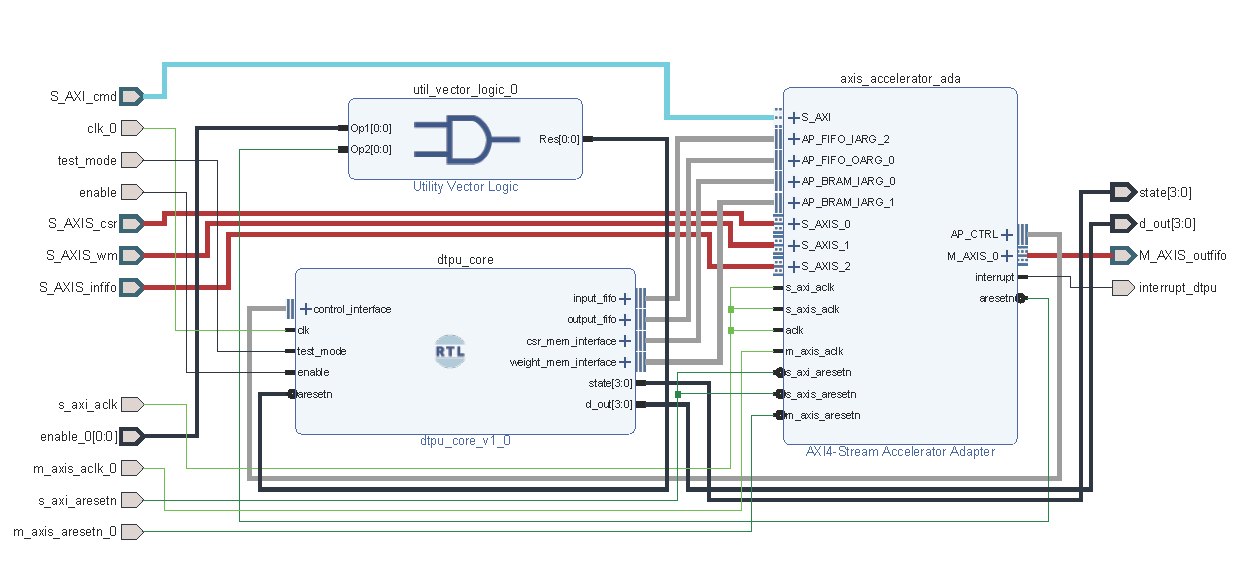
\includegraphics[scale=0.8,angle=0]{./figure/accelerator_schematic.png}
\caption{Real RTL view of DTPU accelerator}
\label{fig:rtlaccel}
\end{figure} 
The latter has allowed to completely focus the work on the DTPU core\footnote{See Appendix B}, which has become:
\begin{figure}[H]
\centering
\captionsetup{justification=centering}
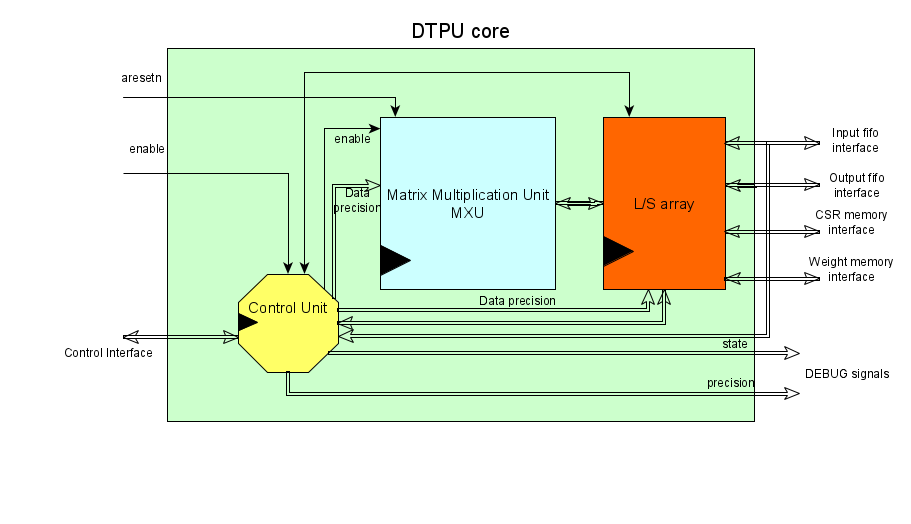
\includegraphics[scale=0.45,angle=0]{./figure/dtpu_core.png}
\caption{RTL view of DTPU core}
\label{fig:dtpucore}
\end{figure} 
Where the sub-units:
\begin{itemize}
\item L/S array provides the data for the Matrix Multiplication Unit, especially the weight data are reused across several executions and therefore loaded once.
\item Control Unit is in charge of handling handshake signals for transferring the ownership of the data (data transferred by the DMA from the Main Memory), load the weights and activation in the respectively units and save the results to the output FIFO. Since it is a Data flow architecture, there is no control flow of the data in the core and this has allowed to keep the Control Unit as simple as possible.
\item Matrix Multiplication Unit (Mxu) is the computation unit of the hardware accelerator. It executes the tensor convolution for different arithmetic precision.
\end{itemize}
\newpage

\subsection{High Level State Machine of Control Unit}
The Dataflow architecture has allowed to design a Control unit as much simple as possible, presented in the below figure:
\begin{figure}[H]
\centering
\captionsetup{justification=centering}
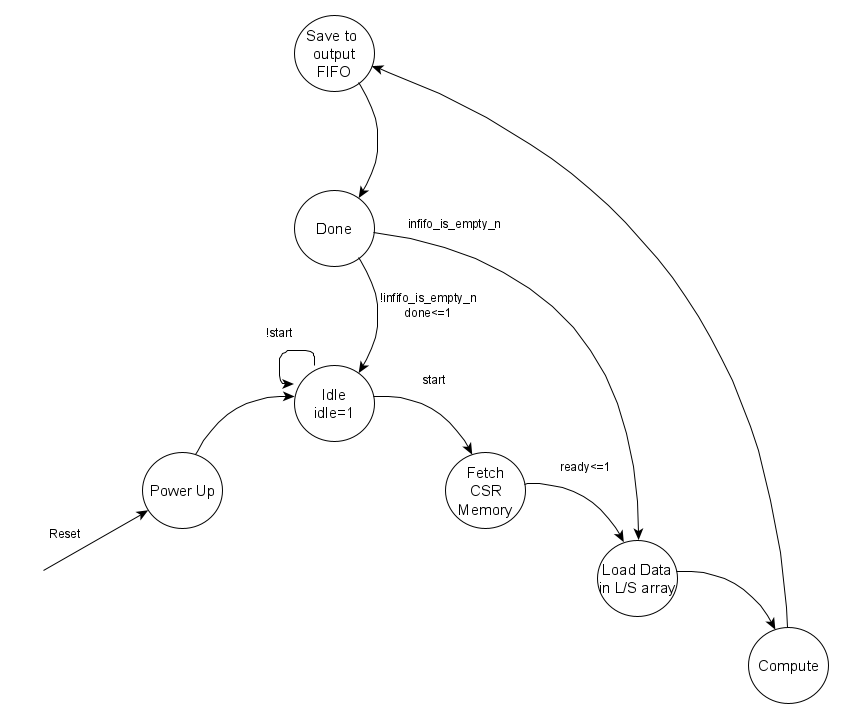
\includegraphics[scale=0.5,angle=0]{./figure/cu.png}
\caption{A high level view of Control Unit}
\label{fig:cu}
\end{figure} 
In which:
\begin{itemize}
\item \textit{Idle} state is waiting for the start signal from the \textit{axis accelerator adapter} (generated when all the data have been transferred\footnote{Input Data, Weight data and CSR data}).
\item \textit{Fetch CSR Memory} state is in charge of retrieving from the CSR memory the desired data precision for the computation and the starting address of the weight memory. It also notifies to the \textit{axis accelerator adapter} that it is ready\footnote{The ready signal is used as handshake between the core and the axis accelerator adapter for transferring the ownership of the data}.
\item \textit{Load data in L/S array} state loads the correct weight values (retrieved from the weight memory) and the activation data into the correct L/S unit. The number of active L/S unit is computed at run time. It depends on from the current required data precision and the fixed number of rows and columns in the MXU.
\item \textit{Compute} state activates the MXU and it waits the end of computation before committing the results to the output FIFO.
\item \textit{Save to output FIFO} state saves the data stored in the active L/S units to the output FIFO.
\item \textit{Done} state, depending on the input FIFO if it is empty or not, continues the computation for the next activation data or it returns to the idle state, notifying to the axis accelerator adapter the end of the computation\footnote{the notification for the end of computation allows the axis accelerator adapter to put the results on the output master axi stream interface in order to be transferred by the DMA}.
\end{itemize}


\subsection{Datapath}
As it is well-known, the execution of ML models is memory intensive and it consists in massive multiplication and accumulation operations. In addition, it can be seen that during execution of ML models some memory location are accessed frequently. Therefore, it is evident that a DataFlow architecture which could exploit local data reuse and compute, massively, in parallel multiplications and additions could boost the performance.
The DTPU core has been designed according to the previously mentioned ideas.
The datapath of the core is presented in Figure \ref{fig:datapath} as block diagram.
\begin{figure}[H]
\centering
\captionsetup{justification=centering}
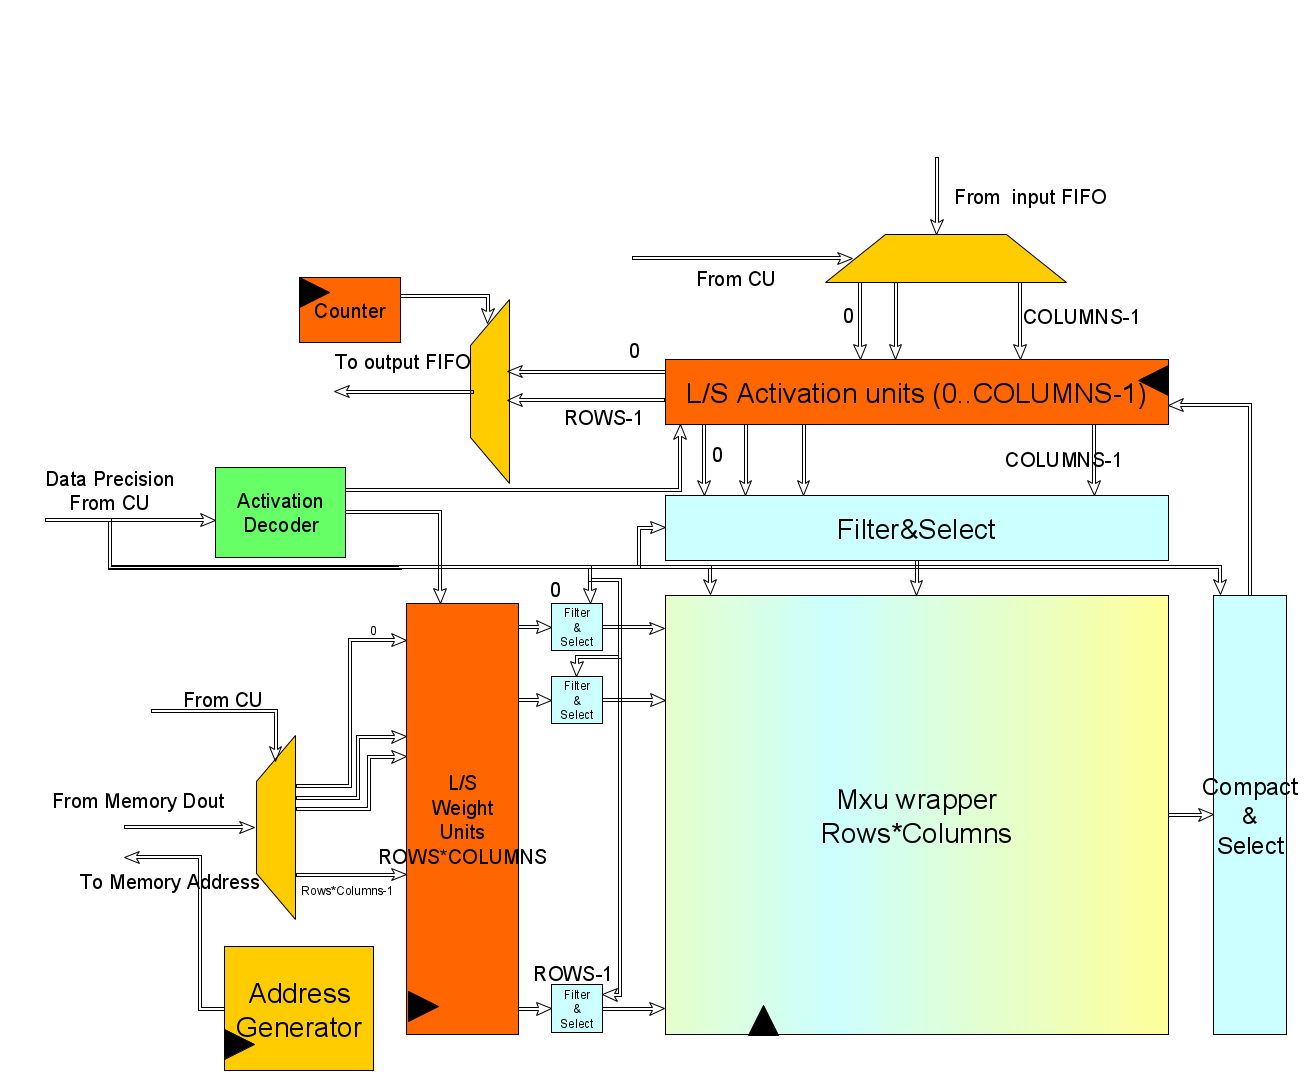
\includegraphics[scale=0.3,angle=0]{./figure/datapath_dtpu_core.png}
\caption{A detailed view of the DTPU core datapath. Enable and resets signals for clocked units has been omitted for improving readability. }
\label{fig:datapath}
\end{figure} 

In Figure \ref{fig:datapath}, the brawn of the accelerator is the MXU wrapper, which contains the symmetric matrix of MACs with variable precision. Regarding the other blocks:
\begin{itemize}
\item Activation Decoder: It is able to generate the right activation signals for the L/S units, depending on from the current data precision and MXU size.
\item Muxes and DeMuxes: Their purpose is to feed the right data from/to memory to/from the right units. The counter (from 0 to ROWS-1) in the Mux for the output FIFO is for saving at every clock cycle a data in the FIFO.
\item Filter\&Select: depending on the precision it provides the correct data to the correct computation units.
\item Compact\&Select: it is the complement of the Filter\&Select unit. It is able to compact the output data from the MXU wrapper and feed the store registers.
\item L/S weight Units: the name L/S has been kept for consistency even if it does not have any store process since the weight are only loaded once (stationary weights) and kept until a next full execution. 
\item L/S Activation Units: they are in charge of loading the data from the input FIFO into batteries of Flip-Flops while at the same time they can save the results to submit late in the output FIFO.
\end{itemize}

\subsubsection{Filter\&Select and Compact\&Select}
In principle, for each Processing element in the MXU wrapper a weight and an activation has to be provided (and as consequence it has to be provided from its relative Load Units). However, since the data width of memories and FIFO has been fixed to its maximum, 64 bits, it comes evident that during a computation with 8 bit integer it will fetch(and save for the output FIFO), in case of a 8x8 Mxu Size, 8 values from FIFO and 64 values from the weight memory. In this scenario all the Flip-Flops of the L/S units (both activation and weights) would sample values where the 56 upper bits are always unused leading to a waste of time for the memory accesses and energy for unused data.\\\\A clever solution is to pack data before sending them to the accelerator. Nevertheless, the pack of data requires to internally unpack and, before committing to the output FIFO, pack the results.
Unpacking and packing are done, respectively, by Filter\&Select and Compact\&Select units.
Retrieving the previous example (computation on 8 bit integer, MXU size of 8x8 and 64 bit memory data) and using the approach of unpacking and packing, this leads to use only one L/S unit for activations (8 for the L/S weight units) for both the load and store operation. With one single L/S active unit and 8 bit integer computation, an 8 bit activation data has to be distributed for each column of the MXU, and this is done by the Filter\&Select unit. For committing to output FIFO, results on 8 bit will be compacted in one single data of 64 bit by the Compact\&select.\\

A visual distribution of the data can be seen in Figure \ref{fig:fscs}. The same can be applied for each row of L/S Weigth units.
\begin{figure}[H]
\centering
\captionsetup{justification=centering}
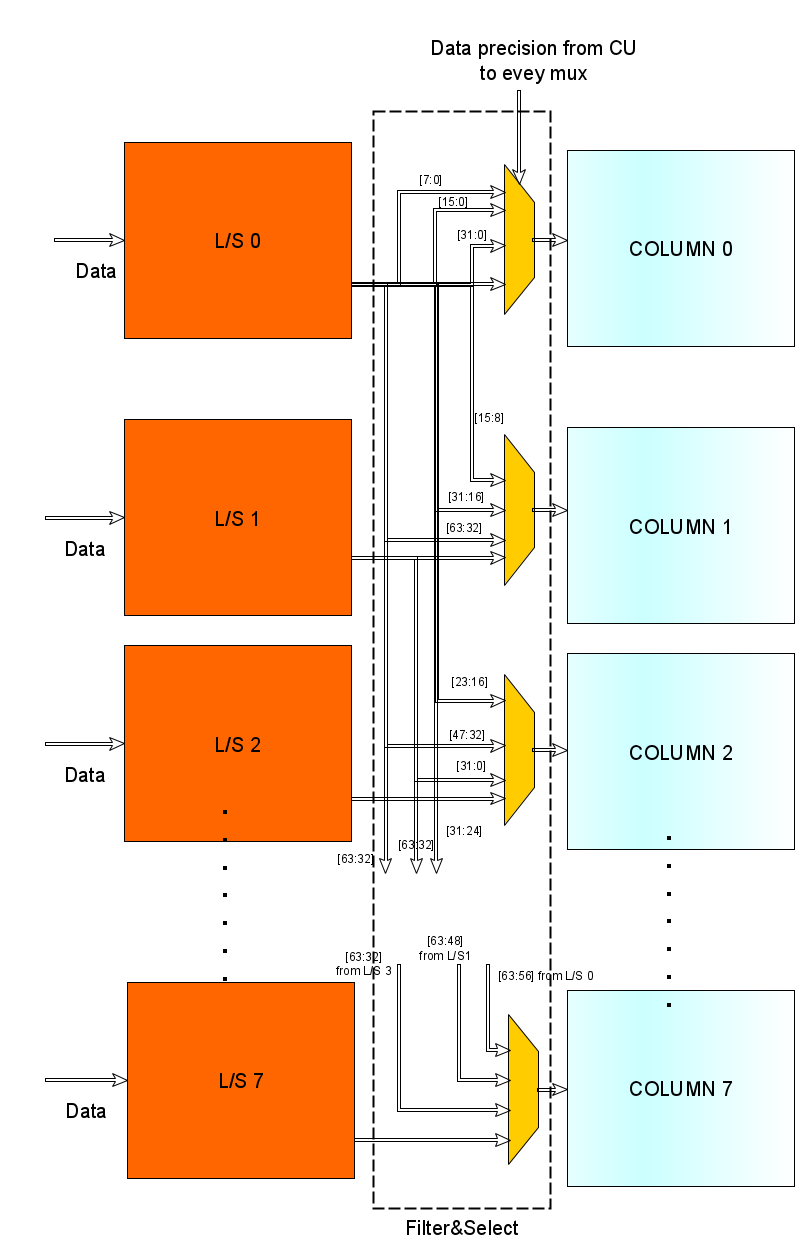
\includegraphics[scale=0.5,angle=0]{./figure/filter_and_select.png}
\caption{Data Distribution of Filter\&Select unit for a MXU size of 8x8}
\label{fig:fscs}
\end{figure} 


In case the required precision is on 16 bit, with the same MXU size, two L/S units for activation are activated (2*ROWS for the L/S weight units) and will feed the respective Columns. The reason behind the two active L/S units is that in 64 bit, only 4 16-bit values can be packed.
Increasing the MXU size, the L/S units are activated accordingly. For example, in case of a MXU size of 16x16 and integer 8 bit, two L/S units are activated (in case of integer 16 computation,4 units are activated).
\\\\
This approach comes also with the overhead of packing and unpacking the data on the CPU but, on the other hand, the memory data movement is reduced and bandwidth increased, with a reduction in the energy consumption (thanks also to the reduced active L/S units).


It is also worth to mention that using size for the MXU which are power of two would maximize the memory bandwidth.

\newpage
\subsubsection{Matrix Multiplication Unit}
The Matrix Multiplication Units (referred as MXU) is the muscle part of the accelerator, where the convolution is done.
As the name suggest, it is organized as a Matrix:
\begin{figure}[H]
\centering
\captionsetup{justification=centering}
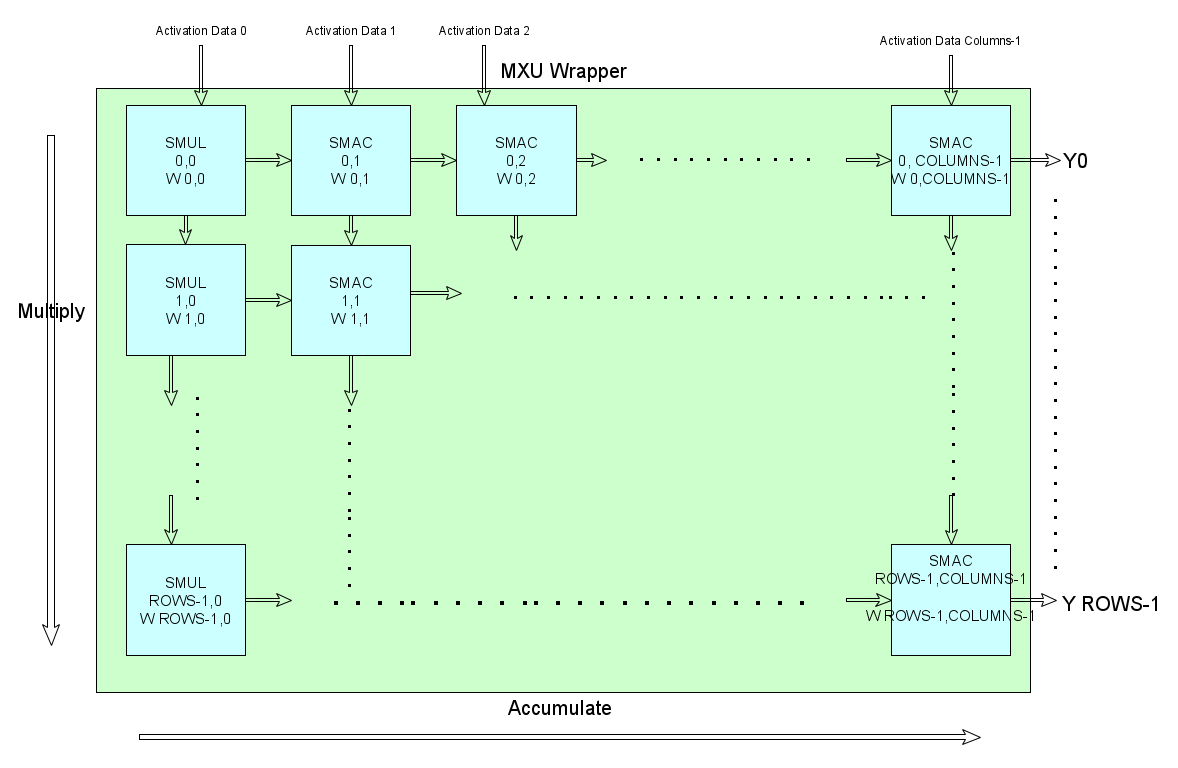
\includegraphics[scale=0.35,angle=0]{./figure/mxu.png}
\caption{MXU interal structure and weights distribution}
\label{fig:mxu}
\end{figure} 

Every sub units has its own weight value (distributed thanks to the L/S weight combined with Filter\&Select units, see Figure \ref{fig:datapath}). It is a homogeneous unit, except for the first column, which does not accumulate. In addition, as it can be seen from the block diagram, there is no control flow between every Processing units. There is only data exchange from the previous unit to the next one (for both axis). This matrix configuration of the hardware allows to massive multiply and accumulate at the same time, in particular it can compute:\\
\begin{center}
$MAC_{OPS}= ROWS*COLUMNS $ \textit{per \# clock cycle required for a single unit}\\ with a $Throughput=Rows$
\end{center}
\ \\
The MXU can be synthesized with different criteria.\\ In particular, the Processing Elements can be independently generated for a single data precision, from integer 8/16/32/64 to floating-point 32 or brain floating-point 16, or with some precision at the same time. Then data precision is decided, via software, and properly controlled using signal in Figure \ref{fig:smac}.
\newpage
A detailed view of SMAC (Sub unit Multiply and Accumulate) and SMUL(Sub unit Multiply), the Processing Elements, is given in Figure \ref{fig:smac}.
\begin{figure}[H]
\centering
\captionsetup{justification=centering}
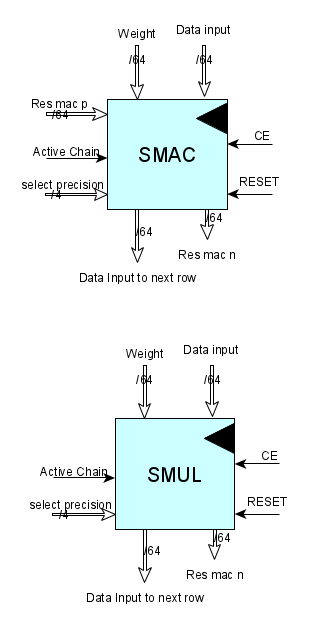
\includegraphics[scale=0.45,angle=0]{./figure/smac.png}
\caption{SMAC and SMUL details}
\label{fig:smac}
\end{figure} 

It is important to mention that the sub units are always receiving data on 64 bits even if internally they may use all of them or not, depending on the value of \textit{select precision} and \textit{active chain} signals. For the full integer configuration (64 bit width operations) beside the possibility of computing for different data width (i.e. choose between 8/16/32/64) the Processing Elements can compute vectorized operations. With the help of \textit{active chain} signal (active low, otherwise it is a 64 bit computation) and data width fixed to 64 bit, it is able to compute at the same time two 8-bit, one 16-bit and one 32-bit operations (multiplication for SMUL and multiplication and addition for SMAC).
However, this comes with the overhead of correctly packing and unpacking the data on the CPU before transferring them to the accelerator.
\newpage
SMAC and SMUL units have been designed, internally, using Vivado DSP primitives \cite{paper:48}, which a general schema can be appreciated in Figure \ref{fig:dsp}:
\begin{figure}[H]
\centering
\captionsetup{justification=centering}
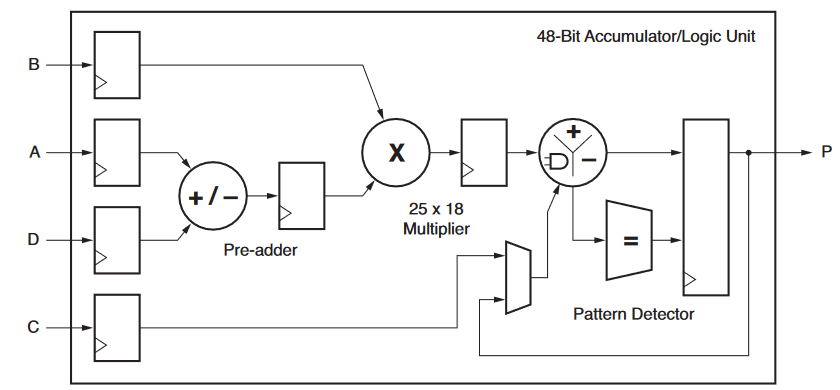
\includegraphics[scale=0.5,angle=0]{./figure/vivado_dsp.png}
\caption{DSP Slice Functionality \cite{paper:48}}
\label{fig:dsp}
\end{figure} 
Allowing fitting two computation (referring to SMAC) in one single unit\footnote{Only for integer 8 and 16} and maximize the resource utilization.\\

As soon as the Synthesis process reach the maximum value of DSP utilization, it does not switch automatically to use Fabric for those primitives. For maximizing the resource usage of the FPGA, the DSP primitives have been regenerated for both Fabric and DSP blocks. In this way, during the generation algorithm for the MXU, it uses primitives for DSP up to the maximum allowed value for the given board and then it starts to utilize Fabric.
This approach has allowed almost a full utilization of the FPGA resources.
